\documentclass[a4paper]{article}

\def\doctitle{实验三\ 放大器的頻率特性研究}

\def\docabstract{}

\def\dockeywords{放大器, 頻率特性}

\usepackage{exp}

\def\doctoc{false}

\begin{document}

%title
\begin{titlepage}
% define titlepage pagenumber (pdf metadata) to "C1"
\renewcommand{\thepage}{C1}
\begin{center}

% title
{\color{fav-red}\rule{\textwidth}{1pt}\par\medskip}
{\huge\bfseries\sffamily \doctitle \par\medskip}
{\color{fav-red}\rule{\textwidth}{1pt}\par\medskip}

% authors and emails
\vspace{1cm}
{\Large\sffamily \scshape \docauthor \par}
\vspace{0.25cm}
{\url{\docemail} \par}

% titlepage logo
\vspace{1cm}

% date and motto
\vfill
{\docdate \par}
{\color{fav-purple}\large\itshape \docmotto \par}

\end{center}
\end{titlepage}

% table of contents
\ifx \doctoc \true
\pagenumbering{roman}
{\sffamily\tableofcontents}
\clearpage
\pagenumbering{arabic}
\fi

%contents here
\section{实验概要}
\subsection{实验目的}
\begin{enumerate}
	\item 研究放大器的頻率特性
	\item 了解計算機仿真技術
\end{enumerate}
\subsection{實驗原理}
\hspace{2em}放大器所放大的信號一般是包含許多頻率成分的複雜信號,含有豐富的諧波,要求放大器對不同頻率分量具有相同的放大能力,才能使放大信號不產生失真。但由於放大器特別是交流放大電路中含有耦合电容、旁路電容、分佈電容及晶體管極間電容等,使放大倍數與信號的頻率有關,這種關系稱為放大器的頻率特性(頻率響應),其中:\par
\begin{enumerate}
    \item 幅頻特性:放大倍數的幅度與頻率的關系;
    \item 相頻特性:放大器對不同頻率的信號會產生不同的相移。
\end{enumerate}
\subsection{實驗儀器和設備}
\begin{enumerate}
    \item AFG3051C 波形發生器
    \item TDS1012C-EDU 數字儲存示波器
    \item SS1792F 可跟踪直流穩定電壓
    \item 電路板
\end{enumerate}
\clearpage
\section{實驗方法和步驟}
\hspace{2em}本實驗的內容是測量單級放大器的幅頻特性和放大器元件對放大器幅頻特性的影響,圖\ref{fig1}為實驗所用電路圖,注意只用右方電電路,因此K2撥向右方。設定信號源的$\rm{V_pp}$值,其中$\rm{Amp} = \SI{500}{\milli\V}$,*示波器顯示為$\SI{250}{\milli\V}$\par
\begin{figure}[H]
    \centering
    %%%%%%%%%%%%%%%%%%%%%%%%%%%%%
    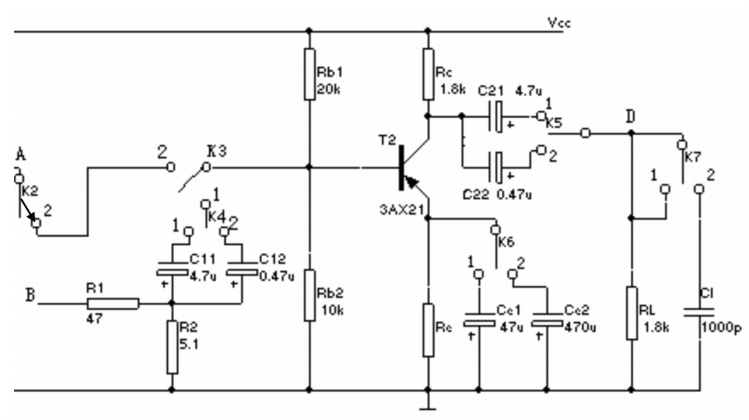
\includegraphics[width=.7\textwidth]{fig1.png}
    \captionsetup{font={normalsize,sf},justification=centering}
    \caption{單級放大器電路號(從講義中修改)}
    \label{fig1}
\end{figure}
\subsection{測量單級放大器的幅頻特性}
\hspace{2em}所用元件為三個電容,*它們的電容值分別為
\begin{enumerate}
    \item $C_1=C_{11}=\SI{4.7}{\micro\F}(\rm{K_4})$
    \item $C_2=C_{21}=\SI{0.47}{\micro\F}(\rm{K_5})$ 
    \item $C_e=C_{e1}=\SI{4.7}{\micro\F}(\rm{K_6})$
    \item 不接$C_L(\rm{K_7})$
\end{enumerate}
    \hspace{2em}在$\rm{B}$點對地輸入正弦信號,從$\SI{5}{\kilo\Hz}$開始向高低端改變輸入信號,記錄$u_o$的幅度。以$\SI{5}{\kilo\Hz}$處及附近平穩值(峰峰值約為$\SI{1250}{\milli\V}$,對應放大倍數$A=\frac{u_o}{u_i}=4.92$)為中頻值,高低截止頻率(下限頻率$f_L$和上限頻率$f_H$)值為$0.707\times\SI{1250}{\milli\V}=\SI{870}{\milli \V}$\par
\subsection{放大器元件對放大幅頻特性的影響}
\begin{enumerate}
    \item 減少$C_1=C_{11}=\SI{0.47}{\micro\F}(\rm{K_4})$
    \item 減少$C_2=C_{21}=\SI{0.47}{\micro\F}(\rm{K_5})$
    \item 增大$C_e=C_{e1}=\SI{470}{\micro\F}(\rm{K_6})$
    \item 在(3)的基礎上,接入$C_L=\SI{1000}{\pico\F}$,增大$C_e$。
\end{enumerate}
\section{實驗數據記錄和分析}
\subsection{測量單級放大器的幅頻特性}
\subsection{放大器元件對放大器幅頻特性影響}
\section{問題討論}
\hspace{2em}(1)为什么测量放大器频率响应所用的示波器或毫伏表都须有足够的频宽?如果被测放大器的频带比所用毫伏表或示波器的频带宽,将出现什么问题?\par
\hspace{2em}(2)用描点法测量放大器的频率响应曲线,有哪些步骤与注意点?为什么要保持放大器的输入信号幅度不变?能不能保持输出电压不变?如果能,怎样测量?\par
\hspace{2em}(3)什么叫通频带,它是如何定义的?怎样求出频带的高低频截止频率 $f_L$ 和 $f_H$?如果不测频率响应曲线,能不能直接测出通频带的高低截止频率?\par
\hspace{2em}(4)級聯後各級放大器靜態工作點有無變化?為甚麼?\par
%%%%%%%%%%%%%%%%%%%%%%%%%%%%%%%%%%%%%%%%%%%%%%%%%%%%%%%%%%%%%%%%%%%

\end{document}